%!TEX root = CS818_assessment.tex
Unsupervised learning is a machine learning technique which seeks to identify patterns and insights in unlabelled data. One common approach to unsupervised learning is cluster analysis, whereby an algorithm sorts unlabelled data into clusters which share some common associations. K-Means clustering employs an algorithm that partitions data into a predetermined number of clusters (defined as K) by iteratively assigning data to a randomly chosen centre known as a centroid. The centroid is then recalculated based on the mean of the data points assigned to it, and the process is repeated until the centroids have stabilised and subsequent recalculations produce similar results \cite{Geron2022}.
 
K-Means can evaluate the behaviour of multiple variables simultaneously, which may permit identification of latent structures or groupings within datasets. As such, it can be used here to uncover distinct profiles of obesity risk that incorporate multiple variables, thereby moving us beyond the uni- and bivariate analyses conducted so far. 

\section{Data preprocessing}
Because K-Means analysis works by calculating the distance between data points, it requires numeric variables. Non-numeric variables must therefore be appropriately encoded. The binary variables 'family\_history\_with\_overweight', 'FAVC', 'SMOKE', and 'SCC', together with 'Gender' (a categorical variable with only two unique answers in the dataset) can be encoded with 1 for 'yes' and 'Male' and 0 for 'no' and 'Female'. 

The dataset also contains two ordinal categories, 'CALC' and 'CAEC', with categories denoting frequency in descending order. These can be encoded such that 'no' = 0, 'Sometimes' = 1, 'Frequently' = 2, and 'Always' = 3. The final non-numerical categories are 'MTRANS' and 'NObeyesdad'. As the options for these variables are not ordinal, the most appropriate encoding method is one-hot, which converts each unique category into a separate binary variable \cite{Geron2022}. This preserves the nominal nature of the variables, and avoids imposing any artificial order on the category options. 

Another important consideration is scaling. With significant variability in the spread across categories, larger scales can end up dominating the clustering process. In this dataset, the scale for weight and to a lesser extent age, have the potential to dominate as captured in \ref{fig:boxplots_prescale}. To avoid distortions, a z-score normalisation has been used to centre those variables around zero with a standard deviation of one. This helps ensure each variable contributes equally to the distance calculations.  

\begin{figure}[h]
\centering
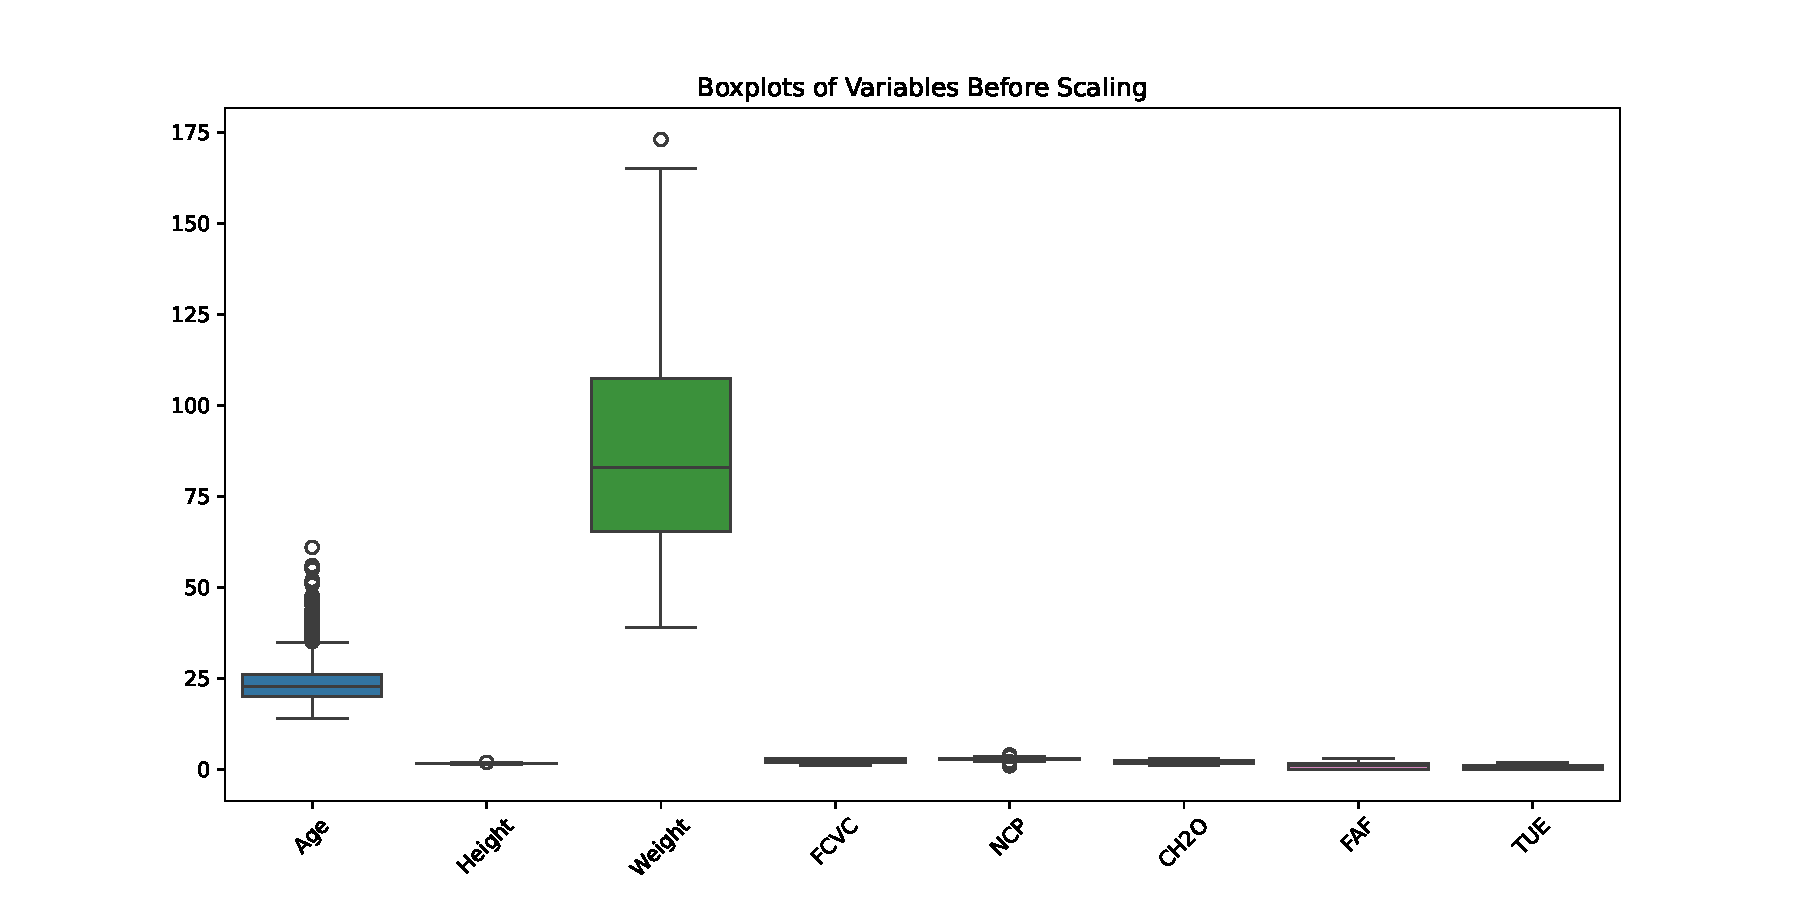
\includegraphics[width=\textwidth]{boxplots_prescale.pdf}
\caption{Boxplots of the dataset's variables before scaling}
\label{fig:boxplots_prescale}
\end{figure}

Finally, Principal Component Analysis has been used to reduce dimensionality. PCA transforms data with potentially correlated variables into a set of uncorrelated variables called principal components, ordered by the amount of variance they capture from the original data. This reduces noise and can make it easier for methods like K-Means to identify patterns. It is particularly effective where datasets have a large number of variables and where variables are likely to be highly correlated as with obesity, height and weight in this dataset \cite{Bandyopadhyay2013}. A condition has been set for the model to use the number of components necessary to capture 95\% of the variance, which ensures the model minimises the loss of potential data patterns.

\section{K-Means: results}

Before the analysis is run, K must be determined. An Elbow plot is used to identify the optimal number of clusters, found at the 'elbow point' where additional clusters no longer significantly reduce inertia. This is used here in conjunction with a Silhouette Score which evaluates cluster cohesion and separation, with higher scores indicating clearer boundaries between clusters \cite{Geron2022}. As can be seen in \ref{fig:elbow_silhouette}, the Elbow plot suggests a change in inertia around k=4, which is also the highest silhouette score, making 4 the best option. 

\begin{figure}[!h]
    \centering
    \begin{subfigure}[b]{0.8\textwidth}
        \centering
        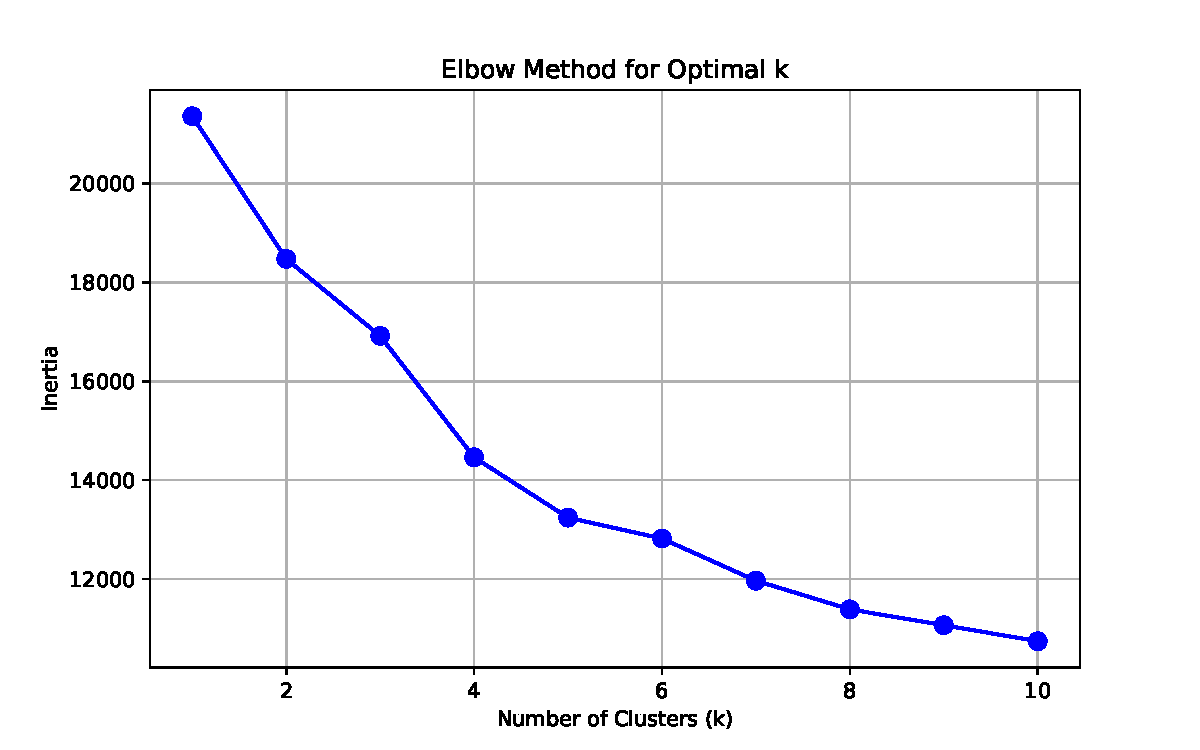
\includegraphics[width=\textwidth]{elbow.pdf}
        \label{fig:elbow}
    \end{subfigure}
    \hfill
    \begin{subfigure}[b]{0.8\textwidth}
        \centering
        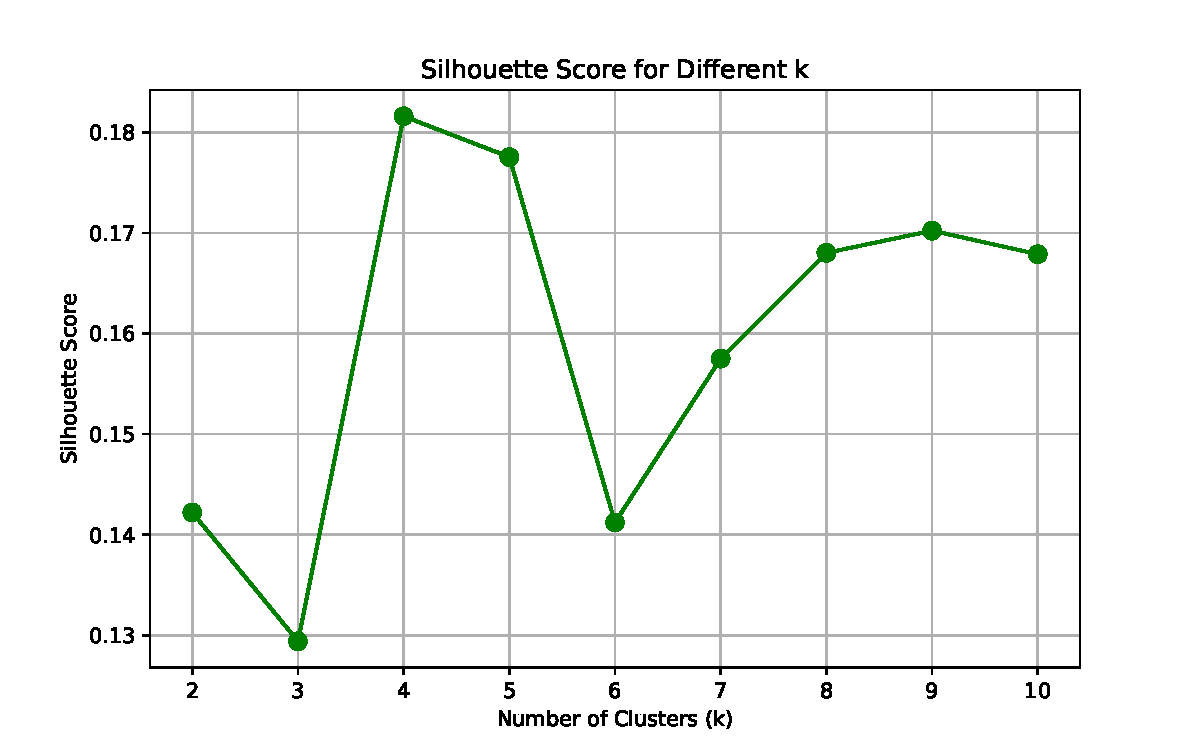
\includegraphics[width=\textwidth]{silhouette.pdf}
        \label{fig:silhouette}
    \end{subfigure}
    \caption{Comparison of Elbow Method and Silhouette Score}
    \label{fig:elbow_silhouette}
\end{figure}

The K-Means analysis was therefore run with k=4. The output cross-tabulated with the obesity categories is shown in \ref{fig:obesity_clusters}, which shows Cluster 0 is most strongly associated with Overweight Level 1, Cluster 1 with Normal Weight, Cluster 2 with Obesity Type III and Cluster 3 with Overweight Level II. The association between Cluster 2 and the highest level of obesity is particularly strong, indicating that analysis has identified a grouping with significant obesity risk. To better understand what characterises each group, \ref{tab:strongest_relationships_minipage} shows the five highest absolute mean values for variables in each cluster, excluding height and weight as the determinants of obesity rates in order to focus in on demographic and lifestyle factors.

Cluster 0 is characterised by few meals but frequent snacking, use of public transport and some prevalence of family obesity. For Cluster 1, frequency of snacking is an even more significant driver, and is coupled with high calorie food consumption. In Cluster 2 the most significant variables are family history and consumption of high calorie food, suggesting both genetic risk and unhealthy eating habits. Frequent snacking also appears and vegetable consumption is also in the top five most significant variables. Finally, in Cluster 3 age is the dominant factor, though family history remains influential, as do high calorie food consumption and frequent snacking. Assessing clusters as a whole, public transport appears frequently, though as addressed earlier in this study, that may reflect the fact that few respondents use alternative methods of transport.

In the next section, supervised analysis is used to generate further insights from the data, before the findings from both analyses are considered in the Discussion section. 

\begin{figure}[h]
    \centering
    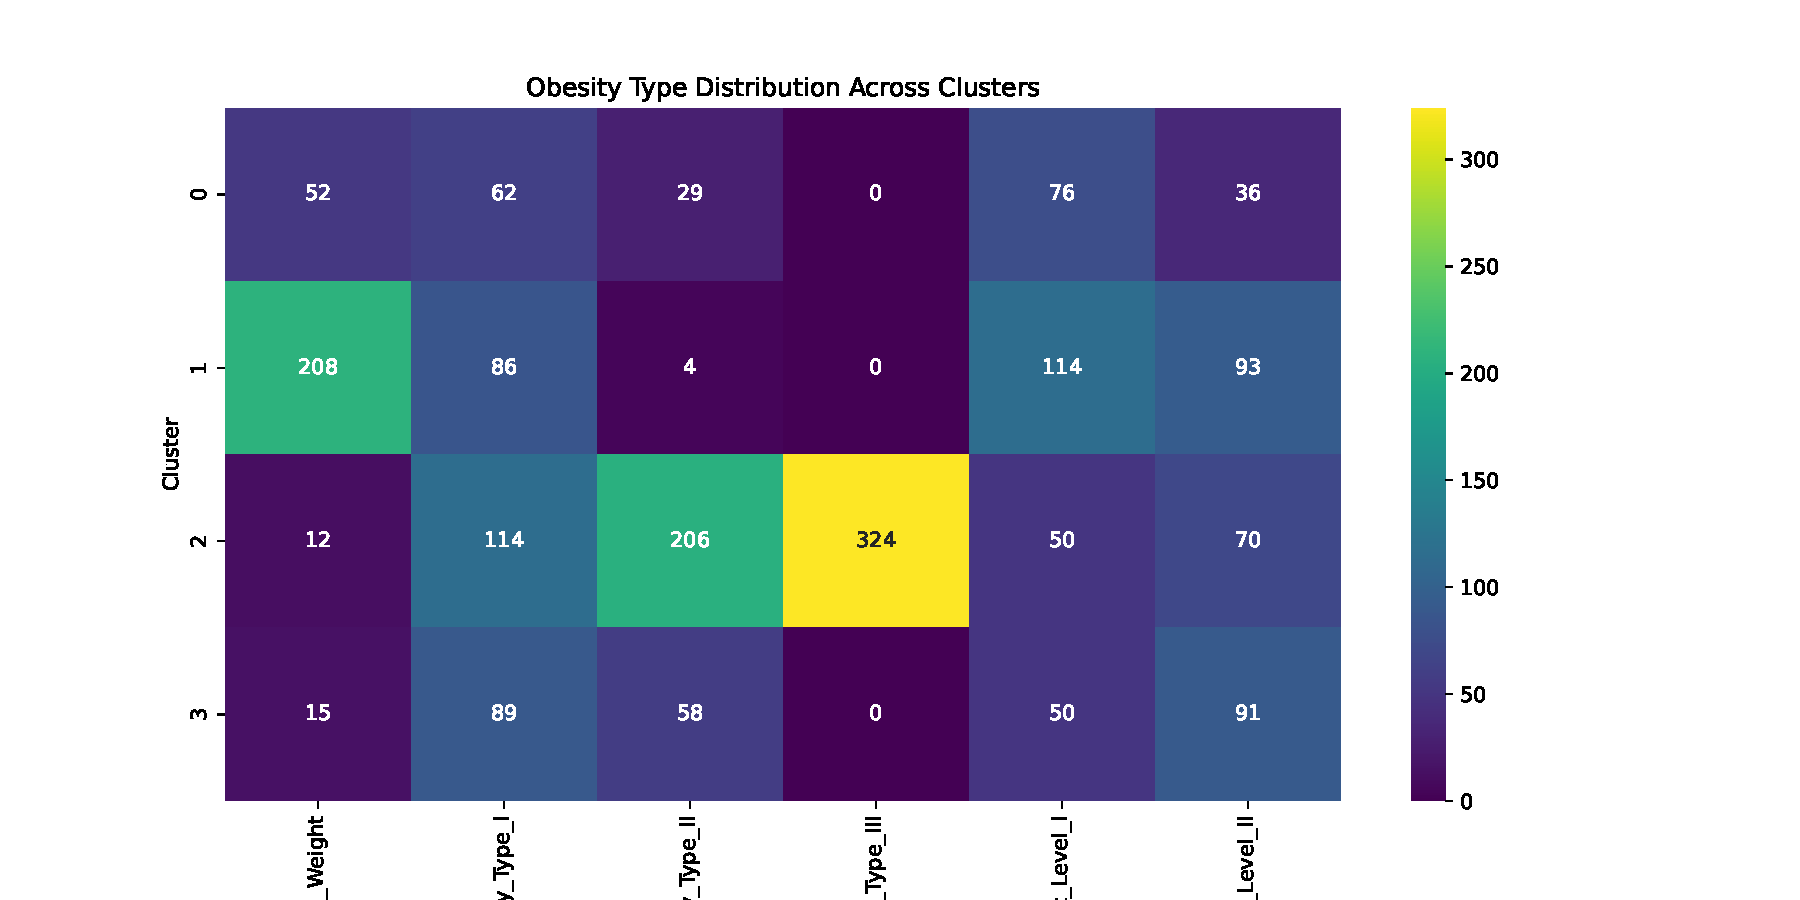
\includegraphics[width=1\textwidth]{obesity_clusters.pdf}
    \caption{Obesity Category Distribution Across Clusters}
    \label{fig:obesity_clusters}
\end{figure}

\begin{table}[h]
\centering
\caption{Top 5 Strongest Relationships per Cluster (Excluding Height, Weight, and Obesity Categories) with Strength Values}
\label{tab:strongest_relationships_minipage}

% ----------- First Row: Cluster 0 and Cluster 1 -----------
\begin{minipage}[t]{0.48\textwidth}
\centering
\caption*{\textbf{Cluster 0}}
\renewcommand{\arraystretch}{1.2}
\begin{tabularx}{\textwidth}{lXr}
\hline
\textbf{Rank} & \textbf{Feature} & \textbf{Strength} \\
\hline
1 & NCP & -1.937 \\
2 & CAEC & 1.110 \\
3 & FAVC & 0.851 \\
4 & Public Transport & 0.929 \\
5 & Family History & 0.640 \\
\hline
\end{tabularx}
\end{minipage}
\hfill
\begin{minipage}[t]{0.48\textwidth}
\centering
\caption*{\textbf{Cluster 1}}
\renewcommand{\arraystretch}{1.2}
\begin{tabularx}{\textwidth}{lXr}
\hline
\textbf{Rank} & \textbf{Feature} & \textbf{Strength} \\
\hline
1 & CAEC & 1.291 \\
2 & Public Transport & 0.812 \\
3 & FAVC & 0.793 \\
4 & NCP & 0.562 \\
5 & Family History & 0.671 \\
\hline
\end{tabularx}
\end{minipage}

% ----------- Second Row: Cluster 2 and Cluster 3 -----------
\begin{minipage}[t]{0.48\textwidth}
\centering
\caption*{\textbf{Cluster 2}}
\renewcommand{\arraystretch}{1.2}
\begin{tabularx}{\textwidth}{lXr}
\hline
\textbf{Rank} & \textbf{Feature} & \textbf{Strength} \\
\hline
1 & Family History & 0.980 \\
2 & FAVC & 0.969 \\
3 & CAEC & 1.043 \\
4 & Public Transport & 0.852 \\
5 & FCVC & 0.338 \\
\hline
\end{tabularx}
\end{minipage}
\hfill
\begin{minipage}[t]{0.48\textwidth}
\centering
\caption*{\textbf{Cluster 3}}
\renewcommand{\arraystretch}{1.2}
\begin{tabularx}{\textwidth}{lXr}
\hline
\textbf{Rank} & \textbf{Feature} & \textbf{Strength} \\
\hline
1 & Age & 1.906 \\
2 & Family History & 0.925 \\
3 & FAVC & 0.912 \\
4 & CAEC & 1.069 \\
5 & Public Transport & 0.154 \\
\hline
\end{tabularx}
\end{minipage}
\end{table}


